\documentclass[final]{beamer}

\usepackage[scale=1.0]{beamerposter}
\usetheme{confposter}

\usepackage{graphicx}
\usepackage{booktabs}
\usepackage{hyperref}
\usepackage{amsmath}
\usepackage{amssymb}
\usepackage{amsfonts}
\usepackage{multirow}
\usepackage{multicol}
\usepackage{listings}
\usepackage{xcolor}
\usepackage[utf8]{inputenc}

\setlength{\paperwidth}{36in}
\setlength{\paperheight}{48in}
\setlength{\topmargin}{-0.5in}

\definecolor{lightgray}{gray}{0.95}

\lstset{
    basicstyle=\ttfamily\small,
    breaklines=true,
    columns=fullflexible,
    frame=single,
    backgroundcolor=\color{lightgray},
    showspaces=false,
    showstringspaces=false,
    language=C++,
    mathescape=false
}

% -------------------------------
% FIXED custom section/subsection
% -------------------------------
\makeatletter
\renewcommand{\section}[1]{%
  \par\vspace{1em}%
  {\noindent\Large\bfseries #1\par}%
  \vspace{0.5em}\hrule\vspace{1em}%
}
\renewcommand{\subsection}[1]{%
  \par\vspace{1em}%
  {\noindent\large\bfseries #1\par}%
  \vspace{0.5em}\hrule\vspace{1em}%
}
\makeatother

\title{C++ QUICK REFERENCE}

\begin{document}

\begin{frame}[t,fragile]

\setlength{\columnseprule}{0.4pt}

\begin{multicols}{4}
\setlength{\columnsep}{1.5cm}

\begin{itemize}
  \item Containers: store collections (\texttt{vector}, \texttt{list}, \texttt{map}, \texttt{set}, \texttt{deque}, ...)
  \item Iterators: traverse containers (input, forward, bidirectional, random-access)
  \item Algorithms: operate on iterator ranges (\texttt{sort}, \texttt{find}, \texttt{for\_each}, ...)
  \item Functors: objects like functions, adapters (\texttt{stack}, \texttt{queue})
\end{itemize}

\subsection{\texttt{std::vector}}

Dynamic contiguous array.

\begin{center}
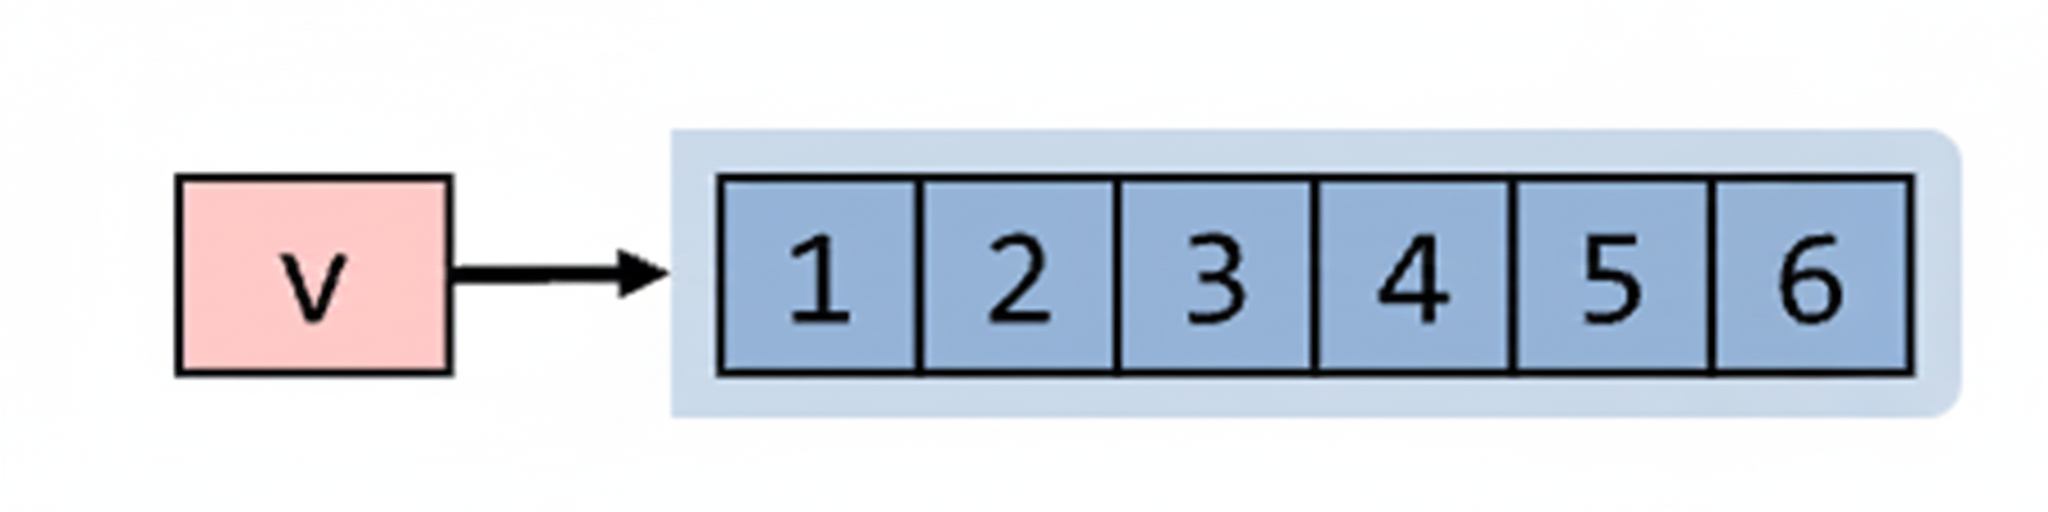
\includegraphics[width=\linewidth]{vector.png}
\end{center}

\begin{lstlisting}
#include <vector>
#include <iostream>

int main() {
    std::vector<int> v;
    for (int i = 0; i < 5; ++i) v.push_back(i*10);

    for (std::vector<int>::size_type i = 0; i < v.size(); ++i)
        std::cout << v[i] << " ";
    std::cout << '\n';

    for (std::vector<int>::iterator it = v.begin(); it != v.end(); ++it)
        std::cout << *it << " ";
    std::cout << '\n';
}
\end{lstlisting}

\subsection{\texttt{std::list}}

Doubly-linked list.

\begin{lstlisting}
#include <list>
#include <iostream>

int main() {
    std::list<int> L;
    L.push_back(1); L.push_back(2); L.push_back(3);
    for (std::list<int>::const_iterator it = L.begin(); it != L.end(); ++it)
        std::cout << *it << " ";
}
\end{lstlisting}

\subsection{Associative containers}

\begin{lstlisting}
#include <map>
#include <string>
#include <iostream>

int main() {
    std::map<std::string, int> ages;
    ages["Alice"] = 30;
    ages["Bob"] = 25;

    for (std::map<std::string,int>::const_iterator it = ages.begin(); it != ages.end(); ++it)
        std::cout << it->first << ": " << it->second << '\n';
}
\end{lstlisting}

\subsection{Container adapters}

\begin{lstlisting}
#include <queue>
#include <iostream>

int main() {
  std::queue<int> q;
  q.push(1);
  q.push(2);
  q.push(3);

  while (!q.empty()) {
    std::cout << q.front() << " ";
    q.pop();
  }
  std::cout << '\n';
}
\end{lstlisting}

\subsection{Unordered maps and pairs}

\begin{lstlisting}
#include <map>
#include <string>
#include <utility>
#include <iostream>

int main() {
  std::map<std::string,int> ages;
  ages.insert(std::make_pair(std::string("Alice"), 30));
  ages.insert(std::make_pair(std::string("Bob"), 25));

  for (std::map<std::string,int>::const_iterator it = ages.begin(); it != ages.end(); ++it)
    std::cout << it->first << ": " << it->second << '\n';

  // If your implementation provides unordered_map:
  /* #include <unordered_map>
     std::unordered_map<std::string,int> um;
     um["Alice"] = 30;
  */
}
\end{lstlisting}

\section{Iterators}

\begin{lstlisting}
#include <vector>
#include <algorithm>
#include <iostream>

int main() {
    std::vector<int> v;
    v.push_back(3); v.push_back(1); v.push_back(2);
    std::sort(v.begin(), v.end());
    for (std::vector<int>::const_iterator it = v.begin(); it != v.end(); ++it)
        std::cout << *it << ' ';
}
\end{lstlisting}

\section{Algorithms}

\subsection{Remove-Erase Idiom}

\begin{lstlisting}
#include <vector>
#include <algorithm>

int main() {
    std::vector<int> v;
    v.push_back(1); v.push_back(2); v.push_back(3); v.push_back(2);
    v.erase(std::remove(v.begin(), v.end(), 2), v.end());
}
\end{lstlisting}

\subsection{Transform and Accumulate}

\begin{lstlisting}
#include <vector>
#include <algorithm>
#include <numeric>
#include <iostream>

struct Square { int operator()(int x) const { return x*x; } };

int main() {
    std::vector<int> v;
    v.push_back(1); v.push_back(2); v.push_back(3);
    std::vector<int> squares(v.size());
    std::transform(v.begin(), v.end(), squares.begin(), Square());
    int sum = std::accumulate(squares.begin(), squares.end(), 0);
    std::cout << "sum = " << sum << '\n';
}
\end{lstlisting}

\section{Functors and Comparators}

\begin{lstlisting}
#include <string>
#include <vector>
#include <algorithm>

struct ByLength {
    bool operator()(const std::string& a, const std::string& b) const {
        return a.size() < b.size();
    }
};

int main() {
    std::vector<std::string> v;
    v.push_back("apple"); v.push_back("kiwi"); v.push_back("banana");
    std::sort(v.begin(), v.end(), ByLength());
}
\end{lstlisting}

\section{Useful Idioms}

\begin{itemize}
  \item Use \texttt{reserve()} on \texttt{vector} when size is known.
  \item Pass large containers by \texttt{const\&}.
  \item Use \texttt{lower\_bound} / \texttt{upper\_bound}.
\end{itemize}

\section{Small Example}

\begin{lstlisting}
#include <vector>
#include <algorithm>
#include <iostream>
#include <numeric>
#include <map>
#include <string>

struct SquareFunctor { int operator()(int x) const { return x * x; } };

int main() {
    std::vector<int> v;
    for (int i = 1; i <= 5; ++i) 
          v.push_back(i);

    std::vector<int> sq(v.size());
    std::transform(v.begin(), v.end(), 
                        sq.begin(), SquareFunctor());

    int sum = std::accumulate(sq.begin(), sq.end(), 0);
    std::cout << "sum of squares = " << sum << '\n';

    std::vector<std::string> words;
      words.push_back("apple");
      words.push_back("kiwi");
      words.push_back("banana");
    std::map<int,int> freq;
    for (std::vector<std::string>::const_iterator it =
                          words.begin(); it != words.end(); ++it)
        ++freq[it->size()];

    for (std::map<int,int>::const_iterator it = freq.begin();
                         it != freq.end(); ++it)
        std::cout << "length " << it->first 
                << ": " << it->second << " word(s)\n";
} 
\end{lstlisting}


 \section{C++11}

  \subsection{Type inference: `auto`, `decltype`}

  \begin{lstlisting}
  #include <vector>
  #include <iostream>

  int main() {
    std::vector<int> v = {1,2,3,4};
    for (auto it = v.begin(); it != v.end(); ++it)
      std::cout << *it << ' ';
    std::cout << "\n";

    auto sum = 0;            // int
    decltype(sum) total = 0; // same type as sum
  }
  \end{lstlisting}

   \subsection{Range-based for}

  \begin{lstlisting}
  #include <vector>
  #include <iostream>

  int main() {
    std::vector<int> v = {10,20,30};
    for (auto x : v) std::cout << x << ' ';
    std::cout << '\n';
    for (auto &x : v) x += 1; // modify in-place
  }
  \end{lstlisting}

  \subsection{Lambda expressions}
 
  \begin{lstlisting}
  #include <algorithm>
  #include <vector>
  #include <iostream>

  int main() {
    std::vector<int> v = {3,1,2};
    std::sort(v.begin(), v.end(), [](int a,int b){ return a<b; });
    std::for_each(v.begin(), v.end(), [](int x){ std::cout << x << ' '; });
    std::cout << '\n';
  }
  \end{lstlisting}


   \section{Move Semantics in C++}

  Beginning with C++11, the C++ language introduced \textit{move semantics}, a mechanism enabling efficient transfer of resources from one object to another. Move semantics reduce unnecessary copying of objects that manage heavy resources such as memory buffers, strings, or file handles.

  We provide a detailed and rigorous explanation of move semantics, beginning with value categories and progressing to move constructors, move assignment, and usage recommendations.

  \section{Value Categories and Reference Types}

  Understanding move semantics requires understanding how C++ distinguishes persistent objects from temporary ones.

  \subsection{Lvalues}

  An \textbf{lvalue} refers to an object with a persistent memory location.

  \begin{lstlisting}[language=C++]
  int x = 10;   // x is an lvalue
  \end{lstlisting}

  Lvalues bind to lvalue references:

  \begin{lstlisting}[language=C++]
  T&
  \end{lstlisting}

  \subsection{Rvalues}

  An \textbf{rvalue} is a temporary expression without a stable address.

  \begin{lstlisting}[language=C++]
  10                 // rvalue literal
  x + 5              // rvalue
  std::string("hi")  // temporary
  \end{lstlisting}

  Rvalues bind to rvalue references:

  \begin{lstlisting}[language=C++]
  T&&
  \end{lstlisting}

  \subsection{Why This Matters}

  Temporaries may be safely “moved from,” enabling efficient resource transfers.

  \section{Move Constructors and Move Assignment}

  Classes that manage resources must implement:

  \begin{itemize}
    \item \textbf{Move constructor}
    \item \textbf{Move assignment operator}
  \end{itemize}

  \subsection{Example Class}

  \begin{lstlisting}[language=C++]
  class MyString {
  private:
    char* data;

  public:
    // Constructor
    MyString(const char* s) {
      size_t n = std::strlen(s) + 1;
      data = new char[n];
      std::memcpy(data, s, n);
    }

    // Destructor
    ~MyString() {
      delete[] data;
    }

    // Copy constructor
    MyString(const MyString& other) {
      size_t n = std::strlen(other.data) + 1;
      data = new char[n];
      std::memcpy(data, other.data, n);
    }
  \end{lstlisting}

  \subsection{Move Constructor}

  \begin{lstlisting}[language=C++]
    MyString(MyString&& other) noexcept
      : data(other.data)
    {
      other.data = nullptr;
    }
  \end{lstlisting}

  \subsection{Move Assignment Operator}

  \begin{lstlisting}[language=C++]
    MyString& operator=(MyString&& other) noexcept {
      if (this != &other) {
        delete[] data;
        data = other.data;
        other.data = nullptr;
      }
      return *this;
    }
  };
  \end{lstlisting}
 
 
\end{multicols}

\end{frame}

\end{document}
